\documentclass[12pt]{article} % \documentclass{} is the first command in any LaTeX code.  It is used to define what kind of document you are creating such as an article or a book, and begins the document preamble

\usepackage{amsmath} % \usepackage is a command that allows you to add functionality to your LaTeX code

\usepackage[papersize={216mm,330mm},tmargin=20mm,bmargin=20mm,lmargin=20mm,rmargin=20mm]{geometry}
\usepackage[english]{babel}
\usepackage[utf8]{inputenc}
\usepackage{amsmath,amssymb,mathabx,amsthm}%\for eqref
\usepackage{mathabx}
\usepackage{lscape}
\usepackage{graphicx}
\usepackage{tikz}\usetikzlibrary{arrows.meta,calc} %library tikz
\usepackage{subcaption}


\usepackage{pgfplots}
\pgfplotsset{compat=1.15}
\usepackage{mathrsfs}
\usetikzlibrary{arrows}
\usepackage{pstricks}
\usepackage{multido}
\usepackage{pst-plot}
\usepackage{rank-2-roots}
\usepackage{color,soul} %package for highlining
\usepackage[colorinlistoftodos]{todonotes}
\usepackage{fancyhdr}
\usepackage{hyperref} %creat hyperlink
\hypersetup{
    colorlinks=true,
    linkcolor=blue,
    filecolor=magenta,      
    urlcolor=cyan,
    pdftitle={Overleaf Example},
    pdfpagemode=FullScreen,
    } %set up a hyperlink to be in blue 
\newtheorem{definition}{Definition}[section]
\newtheorem{theorem}[definition]{Theorem}
\newtheorem{prop}[definition]{Proposition}
\newtheorem{lemma}[definition]{Lemma}
\newtheorem{example}[definition]{Example}

\newtheorem*{remark}{Remark}

\pagestyle{fancy}
\cfoot{\thepage} % this is for the page numbering
\setlength\parindent{0pt} % noindent for the whole document.
\renewcommand{\baselinestretch}{1.1} % increase the distance between line.

\DeclareMathOperator{\SLn}{\text{SL}_n(\mathbb{R})}
\DeclareMathOperator{\GLn}{\text{GL}_n(\mathbb{R})}
\DeclareMathOperator{\slnz}{SL_n(\mathbb{Z})}
\DeclareMathOperator{\glnz}{GL_n(\mathbb{Z})}
\DeclareMathOperator{\vol}{vol}
\DeclareMathOperator{\Hom}{Hom}
\DeclareMathOperator{\fg}{\mathfrak{g}}
\DeclareMathOperator{\fh}{\mathfrak{h}}
\DeclareMathOperator{\SO}{SO_n(\mathbb{R})}
\DeclareMathOperator{\slnr}{\mathfrak{sl}_n(\mathbb{R})}
\DeclareMathOperator{\Ad}{\text{Ad}}
\newcommand{\tpoint}[1]{\subsection{#1}}

\newcommand{\spoint}{\subsection{}}



\title{CHAPTER II :ROOTS AND WEIGHTS FOR $\SLn$/$\GLn$} % Sets article title
\date{\today} % Sets date for date compiled
\begin{document}
\maketitle
In this chapter, we review some basic theory of roots and weights. We will first recall the
general theory and compute explicit examples for $\SLn$/$\GLn$.
\section{Structure theory}
\subsection{The Cartan subalgebra}
First we need the notion of Cartan subalgebra.
\begin{definition}
    For any Lie algebra $\mathfrak{g}$, a subalgebra $\mathfrak{h}$ of $\fg$ is said to be a \textit{Cartan subalgebra} if it is
    \begin{itemize}
        \item $\fh$ is a nilpotent subalgebra.
        \item It is self-normalizing. In particular, we have $\fh = \left\lbrace x \in \fg : [x,\fg] \subset \fh\right\rbrace$.
    \end{itemize}
\end{definition}
When $\fg$ is a semisimple Lie algebra, we have the following theorem:
\begin{theorem}
    Let $\fg$ be a semisimple Lie algebra over an algebraically closed field $k$ of characteristic $0$ with a subalgebra $\fh$.
    Then $\fh$ is a Cartan subalgebra of $\fg$ if and only if it is a maximal toral subalgebra, i.e., is maximal among all subalgebras
    containing only semisimple elements.
\end{theorem}\todo{add citation.}
\subsection{Root space decomposition}
With respect to some choice of Cartan subalgebra, we have a root space decomposition. In particular, there is a finite set
$\Phi \subset \fh^{*}$ of linear forms on $\fh$, whose elements are called \textbf{roots}, such that
\[\fg = \fh \oplus \left(\bigoplus_{\alpha \in \Phi} \mathfrak{g}_\alpha\right),\]
where $\fg_\alpha = \left\lbrace x \in \fg: [h,x] = \alpha(h)x, \forall h \in \fh\right\rbrace$ for any $\alpha \in \Phi$.
\subsection{A specific example: root space decomposition for $\mathfrak{sl}_n(\mathbb{R})$}
For the semisimple Lie algebra $\slnr$, a typical choice of the Cartan subalgebra is the set
\[\fh = \left\lbrace H= \begin{bmatrix}
        a_1    & 0      & \ldots & 0      \\
        0      & a_2    & \ldots & 0      \\
        \vdots & \vdots & \ddots & \vdots \\
        0      & 0      & \cdots & a_n
    \end{bmatrix}, a_1 + a_2+ \ldots + a_n = 0\right\rbrace\]
With respect to this Cartan subalgebra, we can define the linear function
\[L_i \colon \fh \to \mathbb{R}, \quad H \mapsto L_i(H)= a_i\]
Then the roots are given by $\alpha_{ij} :=L_i - L_j$ for distinct $i,j$. We have the root space decomposition for $\slnr$ as follows:
\[\fg = \fh \oplus \left(\bigoplus\fg_{\alpha_{ij}}\right).\]
For the sake of brevity, we will denote $\alpha_{i,i+1}$ by $\alpha_i$ — these are called \textbf{simple roots}.
\subsection{Roots at group level}
Since the main object in this thesis is the Lie groups, we want to understand how the roots
behave at the group level. The analogue for the Cartan subalgebra is the maximal torus
\[T = \left\lbrace t= \begin{bmatrix}
        a_1    & 0      & \ldots & 0      \\
        0      & a_2    & \ldots & 0      \\
        \vdots & \vdots & \ddots & \vdots \\
        0      & 0      & \cdots & a_n
    \end{bmatrix} :  a_i \ne 0\right\rbrace,\]
Then $T$ acts on $\fg$ by conjugation. Explicitly, we can check that
\[\Ad(t)(E_{ij}) = t_it_j^{-1}E_{ij}\]
Therefore, at the group level, the character $\alpha_{ij}(\text{diag}(t_1,\ldots,t_n))=t_it_j^{-1}$
is a root whenever $i \ne j$. The set
\[\Delta = \left\lbrace \alpha_i\mid i =\overline{1,n}\right\rbrace\]
where
\[\alpha_i \colon T \to \mathbb{R}, t \mapsto \dfrac{t_i}{t_{i+1}}\]
is the set of \textbf{simple roots}.
We can decompose the set of roots into two disjoint subsets, namely
\[\Phi = \left\lbrace \alpha_{ij}, i \ne j\right\rbrace = \Phi_+ \coprod \Phi_{-}\]
where the set $\Phi_+$ comprises $\alpha_{ij}$ for $i<j$ and the remaining roots are in $\Phi_{-}$. The former consists of
\textbf{positive roots} while the latter contains \textbf{negative roots}. We have the following lemma:
\begin{lemma}\label{linear-comb-of-roots}
    Each $\alpha \in \Phi$ can be written uniquely as a linear combination
    \[\alpha = m_1\alpha_1+\ldots+m_{d}\alpha_{d}\]
    with all $m_i \in \mathbb{Z}_{\ge 0}$ or $m_i \in \mathbb{Z}_{\le 0}$. If $\alpha \in \Phi_+$ then all $m_i \ge 0$, otherwise $m_i \le 0$ for all $i$.
\end{lemma}
\subsection{Weights}
\todo{define in terms of Lie algebra}
Another class of linear forms that we are interested in are the \textbf{fundamental weights}. For each fundamental
weight $\lambda_i$, we define
\[\lambda_i \colon T \to \mathbb{R}, \quad\lambda_i(t) = a_1\ldots a_i\]
We have the following
\begin{lemma}\label{linear-comb-of-weights}
    We can write
    \[\lambda_i := r_1\alpha_1 + r_2\alpha_2+\ldots + r_d\alpha_d\]
    where $r_i$ are rational numbers such that $r_i \ge 0$.
\end{lemma}
These coefficients $r_i$ are determined by inverting the Cartan matrix of $\slnr$. Hence we postpone a proof
of this until reviewing the notion of Cartan matrices.
\begin{example}
    When $n=3$, we have the following relations \textcolor{red}{add picture}
    \[\lambda_1 = \dfrac{2}{3}\alpha_1+\dfrac{1}{3}\alpha_2, \quad \lambda_2 = \dfrac{1}{3}\alpha_1+\dfrac{2}{3}\alpha_2\]
\end{example}
\begin{figure}[h]
    \centering
    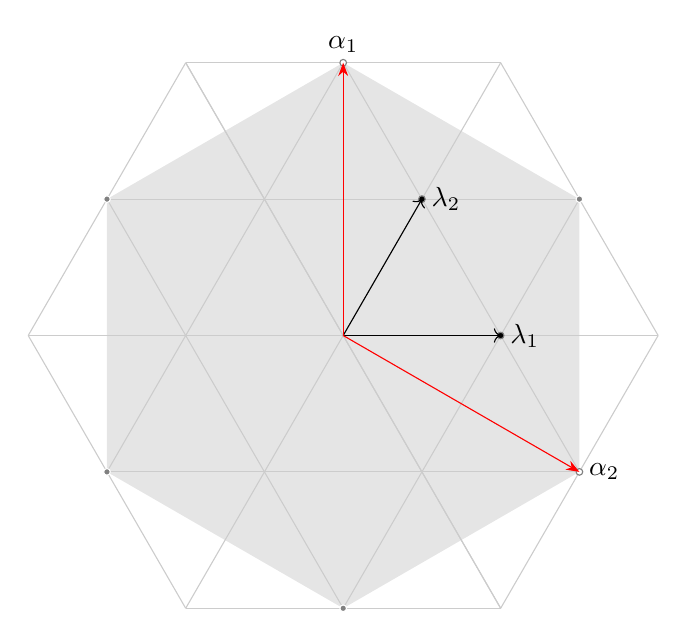
\begin{tikzpicture}
    \begin{rootSystem}[weight length=2cm]{A}
        \roots
        \simpleroots
        \node [above] at \Root {1}{0} {\(\alpha_1\)};
        \node [right] at \Root {0}{1} {\(\alpha_2\)};
        \fundamentalweights
        \node [right] at \weight {1}{0} {\(\lambda_1\)};
        \node [right] at \weight {0}{1} {\(\lambda_2\)};
        \draw[->] (0,0)--\weight{1}{0};
        \draw[->] (0,0)--\weight{0}{1};
        \draw [red, arrows = {-Stealth}] (0,0)--\Root {1}{0};
        \draw [red, arrows = {-Stealth}] (0,0)--\Root {0}{1};
    \end{rootSystem}
\end{tikzpicture}
\caption{Roots and weights for the Lie group $\text{SL}_3(\mathbb{R})$}
\end{figure}


\begin{definition}
    A weight $\lambda$ is called \textbf{dominant} if it satisfies $\left\langle \lambda,\alpha^{\vee} \right\rangle \in \mathbb{Z}_{\ge 0}$ for all $\alpha$.
\end{definition}
Clearly, by lemma \ref{linear-comb-of-roots}, the weight $\lambda$ is dominant if and only if $\left\langle\lambda,\alpha_i^\vee\right\rangle \ge 0$ for all
fundamental roots $\alpha_i$. It is also clear that the set of dominant weights is given by addition of the fundamental weights, namely
\[\Lambda^+ := \left\lbrace c_1\lambda_1+\ldots+c_d\lambda_d \mid c_i \in \mathbb{Z}_{\ge 0}\right\rbrace\]
The set of dominant weights is denoted $\Lambda^+$. A weight $\lambda = \sum n_i \lambda_i$ is called strongly dominant if $n_i > 0$ for all $i$. One important example is the minimal strongly dominant weight given by
\[
    \rho = \sum \lambda_i
\]
This is called the \textbf{Weyl vector} and is characterized in several ways:

\begin{enumerate}
    \item $\left\langle\rho,\alpha_i^\vee\right\rangle = 1$ for all $i$.
    \item
          \[
              \rho = \frac{1}{2} \sum_{\alpha \in \Phi^+} \alpha
          \]
\end{enumerate}

To prove the last equation we use the action of the Weyl group $W$. Let $\mu = \frac{1}{2} \sum \alpha$. Apply the simple reflection $s_i$ given by
\[
    s_i(x) = x - \left\langle x, \alpha_i^\vee\right\rangle \alpha_i
\]
We know that $s_i$ sends $\alpha_i$ to $-\alpha_i$ and permutes the other positive roots. So:
\[
    s_i(\mu) = \mu -  \left\langle \mu, \alpha_i^\vee\right\rangle  \alpha_i
\]
Therefore, $(\mu, \alpha_i) = \mu(h_i) = 1$ for all $i$. So, $\mu = \rho$.

Unlike lemma \ref{linear-comb-of-weights}, if we try to express the fundamental weights in terms of the fundamental roots, we don't always
get positive coefficients. However, it is true that all the coefficients must be integers. In particular, we have
\[\alpha_j = \sum n_j\lambda_j, \quad n_j \in \mathbb{Z}.\]
To put it another way, the root lattice $\mathbb{Z}\Delta$ is contained inside the weight lattice.
\subsection{Weyl group}
We only define the Weyl group explicitly for the group $\SLn$ or $\GLn$. It is a fact that the Weyl groups for
these two Lie groups are the same and equal to $W = S_n$ — the permutation group of $n$ letters.  We recall some basic
observations about this group:
\begin{enumerate}
    \item Every $\sigma \in W$ can be written (non-uniquely) as a product of $w_{i_1} \cdots w_{i_k}$ for some integer $k$. Such a sequence is said to have length $k.$ If $k$ is the minimum, over all such writings, it is called the length of $\sigma$ and written $\ell(\sigma)$. Any expression of length $\ell(\sigma)$ for $\sigma$ is called a reduced expression.

    \item The group $S_n$ is generated by $S$ subject to the following two types of relations:
          \begin{itemize}
              \item (Reflection) $w_i^2=1$ for $i \in I$.
              \item (Braid relations) $w_i \, w_{i+1} \, w_i = w_{i+1}w_i w_{i+1}$ for $i = 1, \ldots, n-2$ and $w_i w_j = w_j w_i$ for $|j -i |\geq 2$.
          \end{itemize}
\end{enumerate}
Note that $W$ acts on $\Hom(H, \mathbb{R}^*)$ in the natural way: $w . \varphi(h) = \varphi(w^{-1} h)$. More explicitly,  $\sigma$ sends $\alpha:= \alpha_{ij}$ to $\alpha_{\sigma(i), \sigma(j)}$. Hence we find that
\[w_i \alpha_j = \begin{cases} - \alpha_i          & \mbox{if } i=j           \\
              \alpha_j            & \mbox{ if } |j - i | > 1 \\
              \alpha_i + \alpha_j & \mbox{ if } |j-i|=1\end{cases} \]
We of course also have an action of $W$ on the weights.  For example, one can verify that
\[ \begin{array}{lcr} s_i(\lambda_i) = \lambda_i - \alpha_i & \text{ and } & s_j(\lambda_i) = \lambda_i \mbox{ for } i \neq j \end{array}.\]
Recall the definition of the Weyl vector $\rho$, we have the following generalized action of the Weyl group on $\rho$:
\[ w \rho = \rho - \sum_{\alpha \in \Delta_{w^{-1}}} \alpha,\]
where \textcolor{red}{check this explicitly}
\[\Delta_{\sigma}:= \{ \alpha \in \Phi_+ \mid \sigma(\alpha) \in \Phi_- \}\]
\subsection{Cartan matrix}
We fix a set of simple roots $\Delta = \left\lbrace \alpha_1,\ldots,\alpha_d \right\rbrace$ and define the matrix
\[A = \begin{bmatrix} \left\langle \alpha_i,\alpha_j^\vee  \right\rangle
    \end{bmatrix}\]
If we let $a_{ij}=  \left\langle \alpha_i,\alpha_j^\vee\right\rangle$ then the Cartan matrix has the following simple properties:
\begin{lemma}
    \hfill
    \begin{itemize}
        \item For any $i$, we have $a_{ii}=2$.
        \item For any $i \ne j$, $a_{ij}$ is a non-positive integer, i.e., $a_{ij} \in \mathbb{Z}_{\le 0}$.
    \end{itemize}
\end{lemma}
We give an explicit example for $\slnr$, which has the root system $A_n$. The corresponding Cartan matrix is
\[A_n = \begin{bmatrix}
        2      & -1     & 0      & 0      & \ldots & 0      \\
        -1     & 2      & -1     & 0      & \ldots & 0      \\
        \vdots & \vdots & \vdots & \vdots & \ddots & \vdots \\
        0      & 0      & \ldots & -1     & 2      & -1     \\
        0      & 0      & \ldots & 0      & -1     & 2      \\
    \end{bmatrix}\]
The Cartan matrix provides a linear combination presentation of the fundamental roots $\alpha_j$ in terms of fundamental weights $\lambda_i$,
as stated in the following lemma:
\begin{lemma}\label{weight-root-comb}
    Fix a number $n$ and consider the set of fundamental roots $\alpha_j$ as well as the set of weights $\lambda_i$ of $\SLn$, we have the following relations
    \[\alpha_i = \begin{cases}
            2\lambda_1-\lambda_2,                    & \mbox{ if } i = 1 \\
            -\lambda_{i-1}+2\lambda_i-\lambda_{i+1}, & \mbox{ if } 1<i<n \\
            -\lambda_{n-1}+2\lambda_n,               & \mbox{ if } i =n
        \end{cases}.\]
\end{lemma}
\begin{proof}
    Note that we have
    \[\left\langle \alpha_i,\alpha_j^{\vee}\right\rangle = \begin{cases}
            2, \mbox{ if } i =j     \\
            -1, \mbox{ if } |i-j|=1 \\
            0, \mbox{ otherwise }
        \end{cases}. \]
    So if we let $\alpha_j = \sum_{i=1}^n a_{ij}\lambda_i$ and compute $\left\langle \alpha_i,\alpha_j^{\vee}\right\rangle$, the result follows immediately.
\end{proof}
We will also need the inverse of the Cartan matrices of type $A_n$. The following formula for the 
inverse matrices of $\slnr$ can be found in \cite{}
\begin{theorem}
The inverse of the Cartan matrices
\[A_n = \begin{bmatrix}
        2      & -1     & 0      & 0      & \ldots & 0      \\
        -1     & 2      & -1     & 0      & \ldots & 0      \\
        \vdots & \vdots & \vdots & \vdots & \ddots & \vdots \\
        0      & 0      & \ldots & -1     & 2      & -1     \\
        0      & 0      & \ldots & 0      & -1     & 2      \\
    \end{bmatrix},\]
    is the matrix $(A_n)^{-1}$ with the entries given by the following formula:
    \[(A_n)^{-1}_{ij} = \min\{i,j\}-\dfrac{ij}{n+1}\]
As a consequence, we can see that the entries for the inverse matrix $(A_n)^{-1}$ are positive. Indeed, assume that 
$i \ge j$, we have 
\[(A_n)^{-1}_{ij} = \dfrac{j(n+1-i)}{n+1}>0\]
In particular, we have just proved lemma $\ref{linear-comb-of-weights}$.
\end{theorem}
\section{Parabolic subgroups}
We shall provide two equivalent viewpoints on parabolic subgroups. They will play different roles in defining
different notions of semi-stability in the next chapter.
\subsection{Parabolic subgroups I: An explicit description}
For our purposes, it is enough to define the standard parabolic subgroups.  There exists a bijection between each parabolic subgroup of $\SLn$
and each partition of $n$. We can therefore define the parabolic subgroup explicitly as follows:
\begin{definition}
    The standard parabolic subgroup associated to the partition $n = n_1 + n_2 + \cdots + n_r$ is denoted $P_{n_1,\ldots,n_r}$ and is defined to be the group of all matrices of the form
    \[
        \begin{bmatrix}
            \mathfrak{m}_1 & 0              & \ldots & 0              \\
            0              & \mathfrak{m}_2 & \ldots & 0              \\
            \vdots         & \vdots         & \ddots & \vdots         \\
            0              & 0              & \ldots & \mathfrak{m}_k
        \end{bmatrix} ,
    \]
    where $\mathfrak{m}_{i} \in \mathrm{GL}(n_i, \mathbb{R})$ for $1 \leq i \leq r$. The integer $r$ is called the rank of the parabolic subgroup $P_{n_1,\ldots,n_r}$.
\end{definition}

\begin{definition}
    The maximal standard parabolic subgroups in $\text{GL}_n(k)$ correspond to the
    stabilizer of the flag of type $\rho_i =(i,n-i)$, where $i = 1,\ldots,n-1$. We will
    further denote $Q_i = P_{\rho_i}$ and $\textbf{MaxParSt}$ the collection of such maximal parabolic subgroups.
\end{definition}

\begin{example}
    Below we list all the standard parabolic subgroups in $\text{GL}_3(\mathbb{R})$ and $\text{GL}_4(\mathbb{R})$.
    \begin{itemize}
        \item For $\text{GL}_3(\mathbb{R})$, there are three standard parabolic subgroups corresponding to
              three partitions of $3$, namely
              \[ 3 = 1+ 1+ 1, \quad 3 =1+2 , \quad 3 = 2+1\]
              For a partition $(r_1,\ldots,r_{s+1})$, we denote $P_{(r_1,\ldots,r_{s+1})}$ the corresponding parabolic subgroup. Thus, we have
              \begin{align*}
                   & P_{1,1,1} = \left\lbrace \begin{bmatrix}
                                                  \ast & \ast & \ast \\
                                                  0    & \ast & \ast \\
                                                  0    & 0    & \ast
                                              \end{bmatrix}\right\rbrace, \quad P_{1,2} =\left\lbrace \begin{bmatrix}
                                                                                                          \ast & \ast & \ast \\
                                                                                                          0    & \ast & \ast \\
                                                                                                          0    & \ast & \ast
                                                                                                      \end{bmatrix}\right\rbrace \\
                   & P_{2,1} = \left\lbrace \begin{bmatrix}
                                                \ast & \ast & \ast \\
                                                \ast & \ast & \ast \\
                                                0    & 0    & \ast
                                            \end{bmatrix}\right\rbrace
              \end{align*}
              Clearly $\textbf{MaxParSt} = \left\lbrace P_{2,1}, P_{1,2}\right\rbrace$.
        \item For  $\text{GL}_4(\mathbb{R})$, there are seven standard parabolic subgroups for seven partitions
              \[ 4 = 1+ 1+1+1, \quad 4 =1+1+2, \quad 4 = 1+2+1\]
              \[4 =2+1+1, \quad 4 = 1+3, \quad 4 = 2+2, \quad 4 = 3+1\]
              Explicitly, we have the following subgroups
              \begin{align*}
                   & P_{1,1,1,1} = \left\lbrace \begin{bmatrix}
                                                    \ast & \ast & \ast & \ast \\
                                                    0    & \ast & \ast & \ast \\
                                                    0    & 0    & \ast & \ast \\
                                                    0    & 0    & 0    & \ast \\
                                                \end{bmatrix} \right\rbrace, \quad & P_{1,1,2} = \left\lbrace \begin{bmatrix}
                                                                                                                  \ast & \ast & \ast & \ast \\
                                                                                                                  0    & \ast & \ast & \ast \\
                                                                                                                  0    & 0    & \ast & \ast \\
                                                                                                                  0    & 0    & \ast & \ast \\
                                                                                                              \end{bmatrix} \right\rbrace \\
                   & P_{1,2,1} = \left\lbrace \begin{bmatrix}
                                                  \ast & \ast & \ast & \ast \\
                                                  0    & \ast & \ast & \ast \\
                                                  0    & \ast & \ast & \ast \\
                                                  0    & 0    & 0    & \ast \\
                                              \end{bmatrix} \right\rbrace, \quad   & P_{2,1,1} = \left\lbrace \begin{bmatrix}
                                                                                                                  \ast & \ast & \ast & \ast \\
                                                                                                                  \ast & \ast & \ast & \ast \\
                                                                                                                  0    & 0    & \ast & \ast \\
                                                                                                                  0    & 0    & 0    & \ast \\
                                                                                                              \end{bmatrix} \right\rbrace \\
                   & P_{1,3} = \left\lbrace \begin{bmatrix}
                                                \ast & \ast & \ast & \ast \\
                                                0    & \ast & \ast & \ast \\
                                                0    & \ast & \ast & \ast \\
                                                0    & \ast & \ast & \ast \\
                                            \end{bmatrix} \right\rbrace, \quad     & P_{3,1} = \left\lbrace \begin{bmatrix}
                                                                                                                \ast & \ast & \ast & \ast \\
                                                                                                                \ast & \ast & \ast & \ast \\
                                                                                                                \ast & \ast & \ast & \ast \\
                                                                                                                0    & 0    & 0    & \ast \\
                                                                                                            \end{bmatrix} \right\rbrace   \\
                   & P_{2,2} = \left\lbrace \begin{bmatrix}
                                                \ast & \ast & \ast & \ast \\
                                                \ast & \ast & \ast & \ast \\
                                                0    & 0    & \ast & \ast \\
                                                0    & 0    & \ast & \ast \\
                                            \end{bmatrix} \right\rbrace
              \end{align*}
              Clearly $\textbf{MaxParSt} = \left\lbrace P_{1,3},P_{3,1},P_{2,2}\right\rbrace.$
    \end{itemize}
\end{example}
\subsection{Parabolic subgroups II: Using BN-pairs}
We first introduce the BN-pairs:
\begin{definition}[BN-pairs]
    A \textbf{BN-pair} is a 4-tuple $(G,B,N,R)$ where $G$ is a group generated by subgroups $B$ and $N$.
    The subgroup $H = B \cap N$, $R$ is a finite set of involutions which generate the \textit{Weyl group} $W= N/H$. Moreover,
    the following theorem holds:
    \begin{itemize}
        \item If $ r \in R$ and $w \in W$, then $rBw \subset BwB \cup BrwB$.
        \item If $r \in R, rBr \ne B$.
    \end{itemize}
\end{definition}
For our purposes, it is enough to concentrate on the following example.
\begin{example}
    Let $G = \GLn$, then the sets $B,N,R$ are given explicitly as follows:
    \begin{itemize}
        \item $B = \text{ upper triangular matrices}$
        \item $N = \text{ monomial matrices, namely, matrices that have exactly one non-zero entry in each row and column}$
        \item From the above, it is clear that $H = B \cap N$ is the diagonal group, and this group is normal in $N$.
        \item It can be shown that $W = N/H \cong S_n$, thus $R = \left\lbrace (i,i-1)\right\rbrace $ — the set of transpositions.
    \end{itemize}
\end{example}
Let $J \subset R$, we define $W_J$ to be the subgroup of $W$ generated by the involutions
$r \in R$. We call it a \textbf{standard parabolic subgroup} of $W$. Set $P_J = BW_JB$ as in the notation of
BN-pairs. We have the following theorem:
\begin{theorem}
    \hfill
    \begin{itemize}
        \item $P_J$ is a subgroup of $G$. In particular, we have
              \[G = BWB,\]
              which is called the \textbf{Bruhat decomposition} of $G$.
        \item If $P_I=P_J$ then we have $I=J$.
        \item All subgroups of $G$ containing $B$ arise in this way. \textcolor{red}{Add proofs?}
    \end{itemize}
\end{theorem}
The above theorem leads to the following definition of parabolic subgroups:
\begin{definition}[Parabolic subgroups]
    Using the same notation in the previous theorem, we call the subgroups $P_J$ with $J \subset R$  \textit{standard parabolic subgroups} of the group $G$.
\end{definition}
We would like to explicitly describe the parabolic subgroups for $\SLn$.
\begin{example}
    As introduced in the previous section, the set $\Phi = \left\lbrace \alpha_{ij}\right\rbrace $ forms a
    root system for $\SLn$. The Borel subgroup is just $B \cap \SLn$, the group of upper triangular matrices with determinant $1$.
    We also consider the set $N$ of monomial matrices  with determinant $1$. Then it is easy to check that
    $N/H$ is the set of all permutation matrices. That is, $N/H$ is generated by the
    matrices of the form \textcolor{red}{see Cambridge}
    \[r_i := \begin{bmatrix}
            I_{i-1} &   &   &           \\
                    & 0 & 1 &           \\
                    & 1 & 0 &           \\
                    &   &   & I_{n-i-1}
        \end{bmatrix}\]
    Via the identification $s_i \mapsto (i,i+1)$, we identify  the Weyl group $W = N/H \cong S_n$. So
    $R = \left\lbrace (i,i+1)| i = 1,2,\ldots,n-1\right\rbrace $. We consider the set
    $I = R \setminus \{r_i\}$ for some $i<n$. The associated parabolic subgroup of
    $W$ is
    \[W_I = \left\langle r_1,r_2,\ldots r_{i-1},r_{i+1},\ldots, r_{n-1} \right\rangle \cong
        S_i \times S_{n-i}\]
    The corresponding parabolic subgroup is
    \[P_{r_i} := P_I = \left\lbrace \begin{bmatrix}
            A & \ast \\
              & B
        \end{bmatrix} \in \SLn: A \in \text{GL}_i, B \in \text{GL}_{n-i}\right\rbrace \]
\end{example}
\subsection{Parabolic sets and parabolic subalgebras}
\begin{definition}
    Given a root system $\Delta$. A \textbf{parabolic subset} $\Delta_P$ is a subset of $\Delta$ such that
    it satisfies the following conditions:
    \begin{enumerate}
        \item For any $\alpha \in \Delta$, at most one of the two elements $\alpha, - \alpha$ is contained in $\Delta_P$.
        \item It is closed, in the sense that, for any two roots $\alpha,\beta \in \Delta_P$ such that $\alpha+\beta$ is a root, then $\alpha+\beta \in \Delta_P$.
    \end{enumerate}
\end{definition}
The parabolic set parametrizes the parabolic subalgebra with the root system $\Delta$, as given in the following theorem:
\begin{theorem}
    Given a semisimple Lie algebra $\mathfrak{g}$ with the root system $\Delta$. There exists a correspondence between
    parabolic subsets $\Delta_P$ of $\Delta$ and the subalgebras of $\mathfrak{g}$ containing the
    Borel subalgebra $\mathfrak{b}$. The correspondence is given by
    \[ \Delta_P \longleftrightarrow \mathfrak{p}:= \mathfrak{b}\oplus \bigoplus_{\alpha \in \Delta \setminus \Delta_P} g_{\alpha}\]
\end{theorem}
\begin{proof}
    We refer to \cite{} for a proof of this fact.
\end{proof}
\begin{example}
    We consider the case $\mathfrak{g} = \mathfrak{sl}_3(\mathbb{R})$. Let's denote
    $\Pi = \left\lbrace \alpha,\beta\right\rbrace$ a basis for the root system of $\mathfrak{g}$. It is clear that
    the set of positive roots is $\Delta_+=\left\lbrace \alpha,\beta,\gamma \right\rbrace$. There are
    4 parabolic sets, corresponding to 4 parabolic subalgebras given as follows:
    \begin{align*}
        \Delta_P = \Delta_+                 & \longleftrightarrow \mathfrak{p} = \mathfrak{b}                               \\
        \Delta_{P} =\Delta \cup \{-\alpha\} & \longleftrightarrow \mathfrak{p} = \mathfrak{b} \oplus \mathfrak{g}_{-\alpha} \\
        \Delta_{P}= \Delta \cup \{-\beta\}  & \longleftrightarrow \mathfrak{p} = \mathfrak{b} \oplus \mathfrak{g}_{-\beta}  \\
        \Delta_P= \Delta                    & \longleftrightarrow \mathfrak{p} = \mathfrak{g}
    \end{align*}
\end{example}

\subsection{Langlands decomposition}
We fix a partition of $n$ as
\[n=n_1+n_2+\ldots+n_k\]
and consider the parabolic subgroup of this type, i.e., the subgroup
\[P_{n_1,\ldots, n_k} = \left\lbrace \begin{bmatrix}
        \mathfrak{m}_1 & \ast           & \ldots & \ast           \\
        0              & \mathfrak{m}_2 & \ldots & \ast           \\
        \vdots         & \vdots         & \ddots & \vdots         \\
        0              & 0              & \ldots & \mathfrak{m}_k
    \end{bmatrix} \right\rbrace\]
where $\mathfrak{m}_i$ is invertible of size $n_i \times n_i$.

This group can be factored as
\[P_{n_1,\ldots, n_k} =M_{n_1,\ldots, n_k}N_{n_1,\ldots, n_k}\]
where
\[N_{n_1,\ldots, n_k} = \left\lbrace \begin{bmatrix}
        I_1    & \ast   & \ldots & \ast   \\
        0      & I_2    & \ldots & \ast   \\
        \vdots & \vdots & \ddots & \vdots \\
        0      & 0      & \ldots & I_k
    \end{bmatrix} \right\rbrace \quad \left(I_k \text{ is the $n_k\times n_k$ identity matrix}\right)\]
and
\[M_{n_1,\ldots, n_k} = \left\lbrace \begin{bmatrix}
        \mathfrak{m}_1 & 0              & \ldots & 0              \\
        0              & \mathfrak{m}_2 & \ldots & 0              \\
        \vdots         & \vdots         & \ddots & \vdots         \\
        0              & 0              & \ldots & \mathfrak{m}_k
    \end{bmatrix} \right\rbrace\]

The subgroup $M_{n_1,\ldots, n_k}$ is called the \textbf{Levi component}. We can further factor this subgroup as
\[M_{n_1,\ldots, n_k} = M'_{n_1,\ldots, n_k} \cdot A_{n_1,\ldots, n_k}\]
with $A_{n_1,\ldots, n_k}$ playing the role of the connected center of $M_{n_1,\ldots, n_k}$:
\[A_{n_1,\ldots, n_k} = \left\lbrace \begin{bmatrix}
        t_1I_1 & 0      & \ldots & 0      \\
        0      & t_2I_2 & \ldots & 0      \\
        \vdots & \vdots & \ddots & \vdots \\
        0      & 0      & \ldots & t_kI_k
    \end{bmatrix} : t_i \ne 0\right\rbrace \]
and
\[M'_{n_1,\ldots, n_k} = \left\lbrace \begin{bmatrix}
        \mathfrak{m}'_1 & 0               & \ldots & 0               \\
        0               & \mathfrak{m}'_2 & \ldots & 0               \\
        \vdots          & \vdots          & \ddots & \vdots          \\
        0               & 0               & \ldots & \mathfrak{m}'_k
    \end{bmatrix} \right\rbrace,\]
where $\det(\mathfrak{m}'_i) = \pm 1$.
\begin{definition}
    For a given parabolic subgroup $P$, the factorization
    \[P = M_P \times A_P \times N_P\]
    as above is called the \textbf{Langlands decomposition}.
\end{definition}
\subsection{P-horospherical decomposition}
Using the Langlands decomposition as well as the Iwasawa decomposition $G= ANK = BK$, we observe
the decomposition
\[G = KP = M_PA_PN_PK \cong M_P \times A_P \times N_P\]
As a consequence, we get
\[X_G  = G/K = X_{M_P} \times A_P \times N_P\]
for $X_{M_P} := M_{P}/(K\cap M_P)$. This is the \textbf{P-horospherical} decomposition of the lattice space $X_G$. In this way,
we can identify  $x \in X_G$ with the triple $(m_P(x), a_P(x),n_P(x))$.
\subsection{On the function $H_P$}
Recall that for the Lie group $\SLn$, we attach to it a root system $\Phi = \left\lbrace \alpha_{i,j}\right\rbrace$ with
\[\Delta = \left\lbrace \alpha_i\mid i \in I \right\rbrace, \quad I = \{1,2,\ldots,n-1\}\]
as the set of fundamental roots. It is a fact that the Weyl group $W$ satisfies
\[W = \left\langle r_{\alpha_i}: i \in I \right\rangle\]
For the sake of brevity, we denote $r_{\alpha_i}:=r_i$. Then for each subset $J \subset I$,
we define the following subset of the Cartan subalgebra $\fh$ of $\slnr$:
\begin{align*}
    \fh(J) & :=\text{span}\{ \alpha^\vee_i, i \in J\}                                       \\
    \fh_J  & := \{H \in \fh: \left\langle \alpha_i,H\right\rangle=0 \mbox{ for } i \in J \}
\end{align*}
By the definition of weights, i.e., $\left\langle \lambda_i,\alpha^\vee_j \right\rangle = \delta_{ij}$, it is immediate
that the subspace $\fh_J$ of $\fh$ is orthogonal to $\fh(J)$ and is generated by the set
\[\fh_J = \text{span}\left\lbrace \lambda^\vee_i: i \notin J\right\rbrace \]
We also write $\lambda^{\vee}_{j,J}$ for the basis of $\fh(J)$ containing the fundamental
weight, namely $\left\langle \alpha_k,\lambda^{\vee}_{j,J}\right\rangle = \delta_{kj}$ for $j,k \in J$. We have
the following easy lemma:
\begin{lemma}\label{coeff-H(J)}
    Let $H \in \fg$ be arbitrary. For $J \subsetneq I$ we have the orthogonal decomposition
    \[H = H(J)+H_J,\]
    where $H(J) \in \fh(J)$ and $H_J \in \fh_J$. If $H = \sum_{i=1}^n p_i\lambda^\vee_i$ then
    \[H(J) = \sum_{i \in J} p_i \lambda^\vee_{i,J}\]
\end{lemma}
\begin{proof}
    Let $H(J) = \sum_{i \in J} c_i \lambda^\vee_{i,J}$, then for $i \in J$
    \[p_i = \left\langle \alpha_i,H \right\rangle =\left\langle \alpha_i,H_J+H(J) \right\rangle = \sum_{i \in J}\left\langle \alpha_i,  c_i \lambda^\vee_{i,J}\right\rangle=c_i \]
    Hence $H(J) = \sum_{i \in J} p_i \lambda^\vee_{i,J}$.
\end{proof}
We know from the previous section that for each standard parabolic subgroup of $G$, it must be of the form
$P_J$ for some subset $J \subset \{1,\ldots,n-1\}$. Therefore, we can define $\fh(P):= \fh(J)$ and $ (\fh)_P:= \fh_J$. We will explain why we define it this way shortly in the next section.

\end{document}
// ...existing code...